\include{tex/headerueb}
\include{tex/header}
\include{tex/info}

\newcommand{\nr}{10}
\lstset{language=matlab}

\begin{document}
\section*{Aufgabe 1 - Hough-Transformation - Geradenerkennung}

Ausgangsbild war ``street'', was wir f\"ur einfachere Weiterverarbeitung
auf eine Zweierpotenz skalierten und entsprechend wei\ss{}/graue Balken
erweiterten.
\begin{figure}[H]
\begin{center}
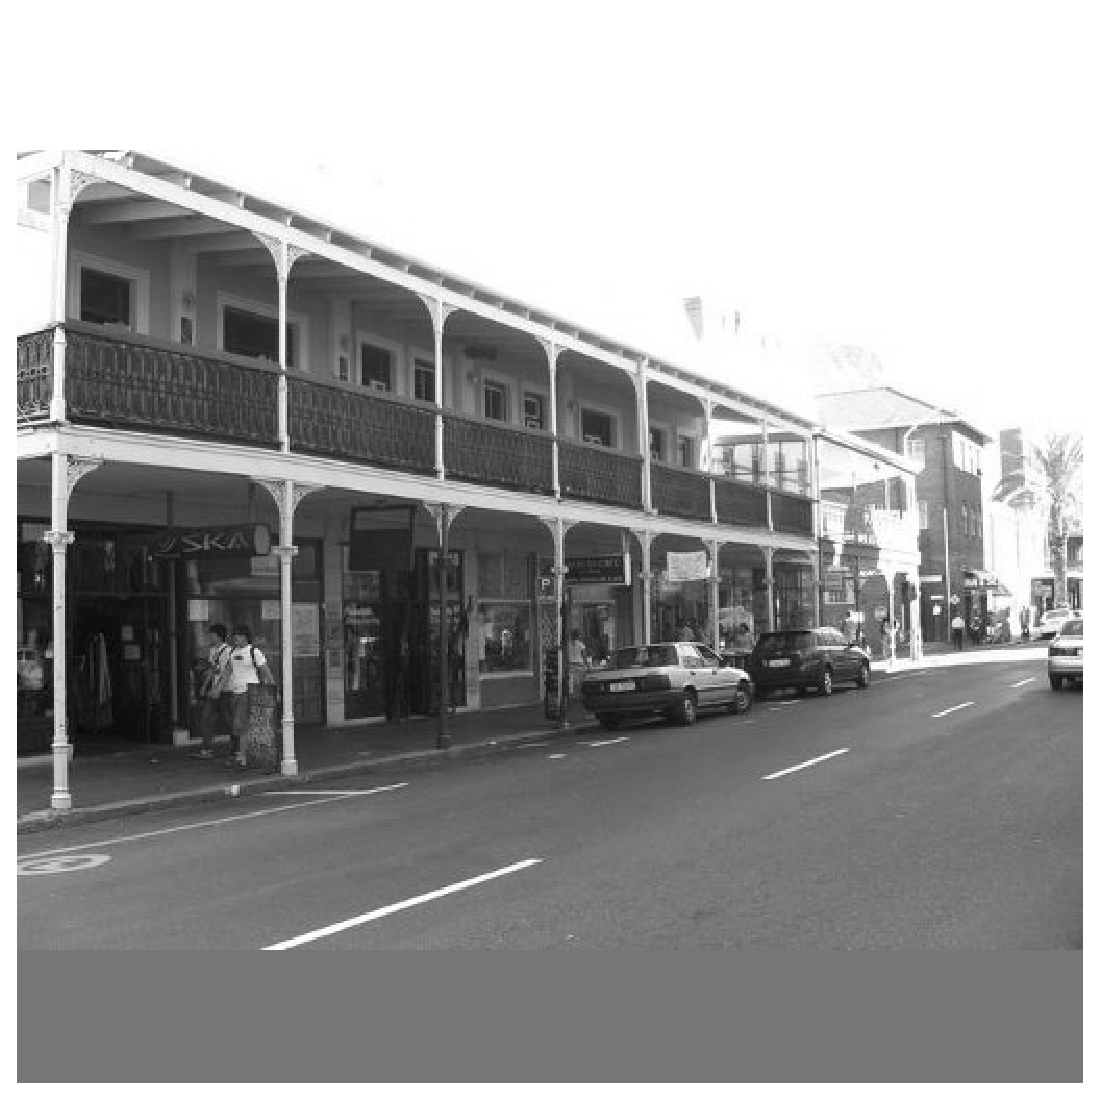
\includegraphics[width=70mm]{u10/street.eps}
\end{center}
\label{street}
\caption{Street - Ausgangsbild}
\end{figure}

Davon ausgehend f\"uhrten wir eine Vorverarbeitung durch. Aus vorhergehenden
U\"bungen verwendeten wir Ableitung nach X- und Y-Richtung (Soebel), berechneten 
den Gradienten (Polarkoordinaten). Zus\"tzlich binarisierten wir das Ergebnis der Gradientenberechnung,
um nur relevante Pixel in die Betrachtung als potentielle Teile einflie\ss{}en zu lassen.

\begin{figure}[H]
\begin{center}
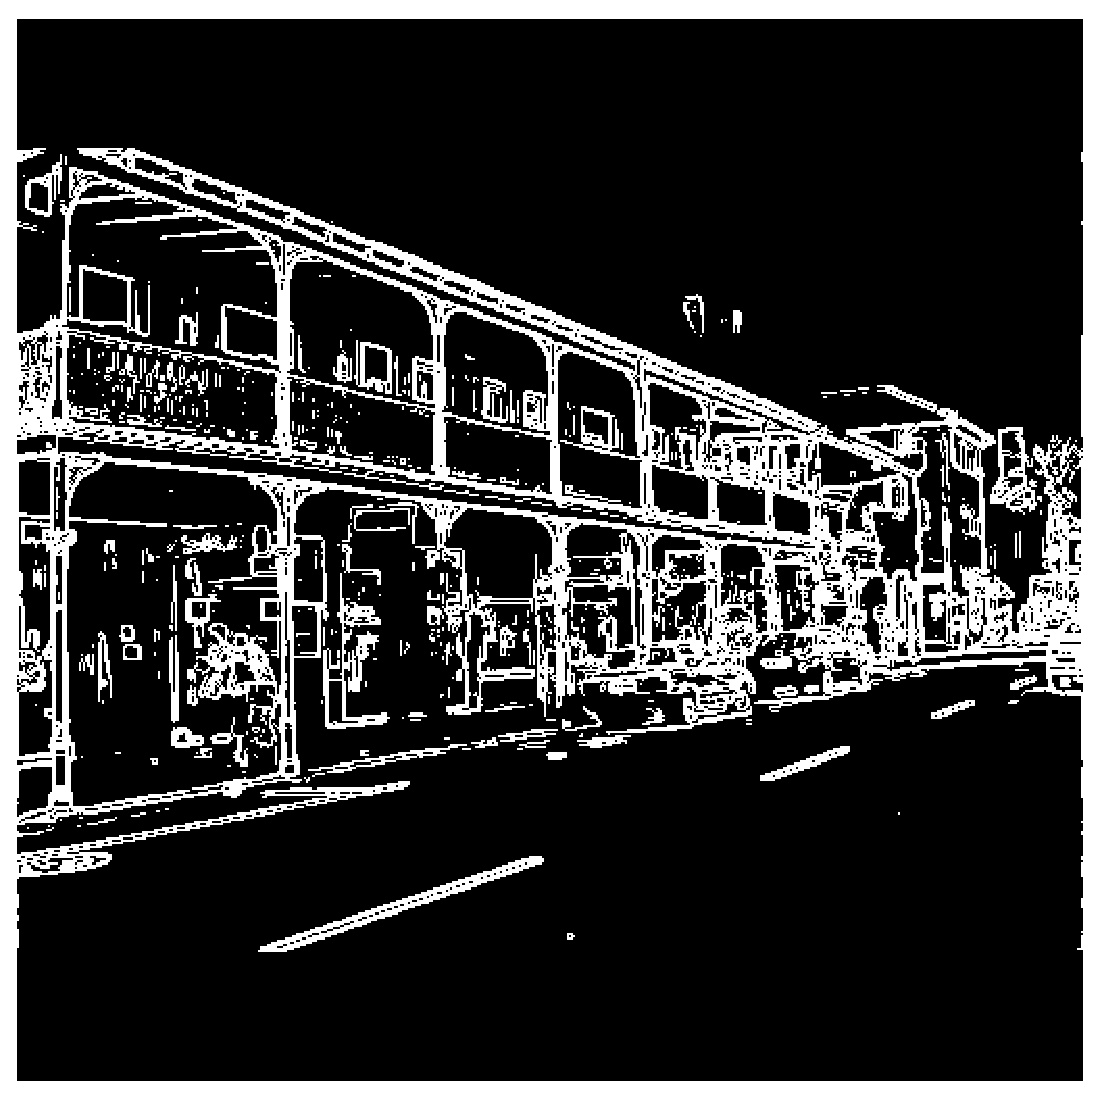
\includegraphics[width=90mm]{u10/street_edges.eps}
\end{center}
\label{streete}
\caption{Nur die Gradienten der wei\ss en Pixel werden betrachtet}
\end{figure}

Im letzten Schritte verwendeten wir den Algorithmus aus der Vorlesung, bei dem 
m\"ogliche Geradenverl\"aufe in Abh\"angigkeit von $d = x \cdot \cos \theta + y \cdot \sin \theta $
betrachtet werden. $\Theta$ geht aus der Gradientenrichtung hervor plus einem zus\"atzlichen
Abweichungsfenster. Die Werte werden diskretisiert und in eine Matrix gespeichert. Die Visualisierung
der Matrix sieht dann wie folgt aus:

\begin{figure} [H]
\begin{center}
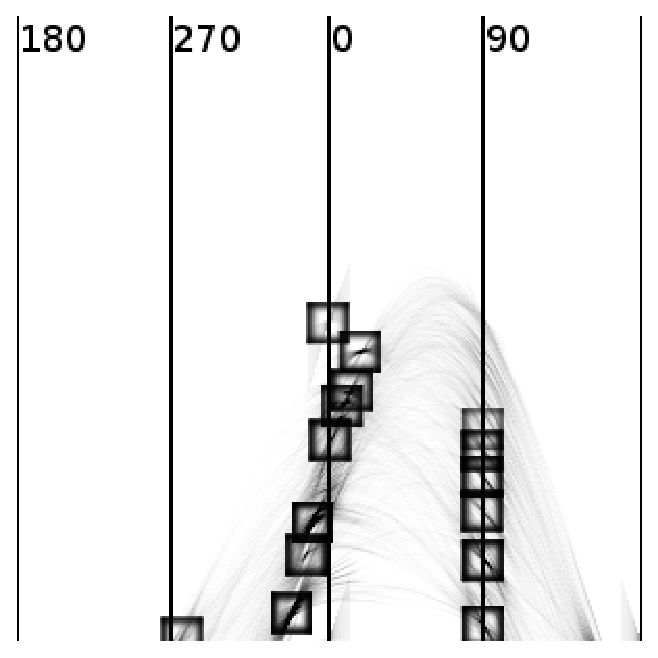
\includegraphics[width=90mm]{u10/lines.eps}
\end{center}
\label{streetl}
\caption{Die erkannten Geraden}
\end{figure}

Interpretation der Grafik: Abbildung von $\theta$ auf $d$, wobei der Nullpunkt in der linken oberen
Ecke liegt. Der Wertebereich von $\theta$ l\"auft von $-\pi$ bis $+\pi$. Zu erkennen sind zwei 
wesentliche Geradenarten. Die mit Variationen um die null Grad und steigendem Abstand (also 
horizontale Linien, die perspektivisch verlaufen) und die Senkrechten, die im geringen Abstandsbereich
dominieren (weil sie auch fl\"achenm\"assig \"uberwiegen) aber in einem konstanten Winkel (90 Grad)
verlaufen.
\\
Anmerkung: W\"ahrend der Erstellung der Matrix mussten wir mehrmals (durch probieren) die
Interpretation der Werte \"andern. Um negative Ds zum Beipsiel zu vermeiden, ist es n\"otig
den Komplementwinkel zu verwenden, wenn nur der Betrag von D verwendet werden soll.

\section*{Aufgabe 2 - Kreiserkennung}
Die Vorverarbeitung laueft wie bei Aufgabe 1 (siehe Abbildung \ref{moon}). Durch
die Verzerrung, Schattierung und Unregelmaessigkeiten der Kraterraender ist das
Ergebnis dieser Vorverarbeitung nicht ideal, aber kleinere kreise sind noch
immer auf der Vroverarbeitenten version zu erkennen.

\begin{figure}[H]
\begin{center}
\includegraphics[width=180mm]{u10/moon.eps}
\end{center}
\label{moon}
\caption{Vorverarbeitung}
\end{figure}

Wie in der Vorlesung vorgestellt, wurden fuer jedes Pixel potentielle
Kreismittelpunkte ($x$ und $y$, Aufloesung $500\times 500$) und Radien ($r \in \{3,\cdots,50\}$) in eine
3D-Matrix eingetragen. Die potentiellen Kreismittelpunkte zu einem Pixel
befinden sich ebenfalls auf einem Kreis mit Radius $r$, sodass alle Stellen mit 
$(x,y) = (r \cos(\theta), r \sin(\theta))$, mit $\theta = [-\pi, \pi]$ gespeichert werden muessen.
Um zu Vermeinden, dass bei einem Durchlauf ueber $\theta$ ein Eintrag in der Matix 2-fach erhoert wird,
werden in einer Hilfsmatrix diejenigen $(x,y)$ makiert, die bei dem Durchlauf schon getroffen wurden.

Abbilung \ref{moons} zeigt 6 durchschnitte durch die Matrix. Maxima sind nicht deutlich und unterscheiden sich kaum von der Umgebung.
Dies zeigt, dass keine eindeutigen Kreise Identivviziert werden konnten, es eher viele moeglich Kreismittelpukte auf dem Bild gibt.
Eine bessere vorverarbeitung waere noetig, um die Krater auf dem Mondoberfaleche eindeutig zu identivizieren.
\begin{figure}[H]
\begin{center}
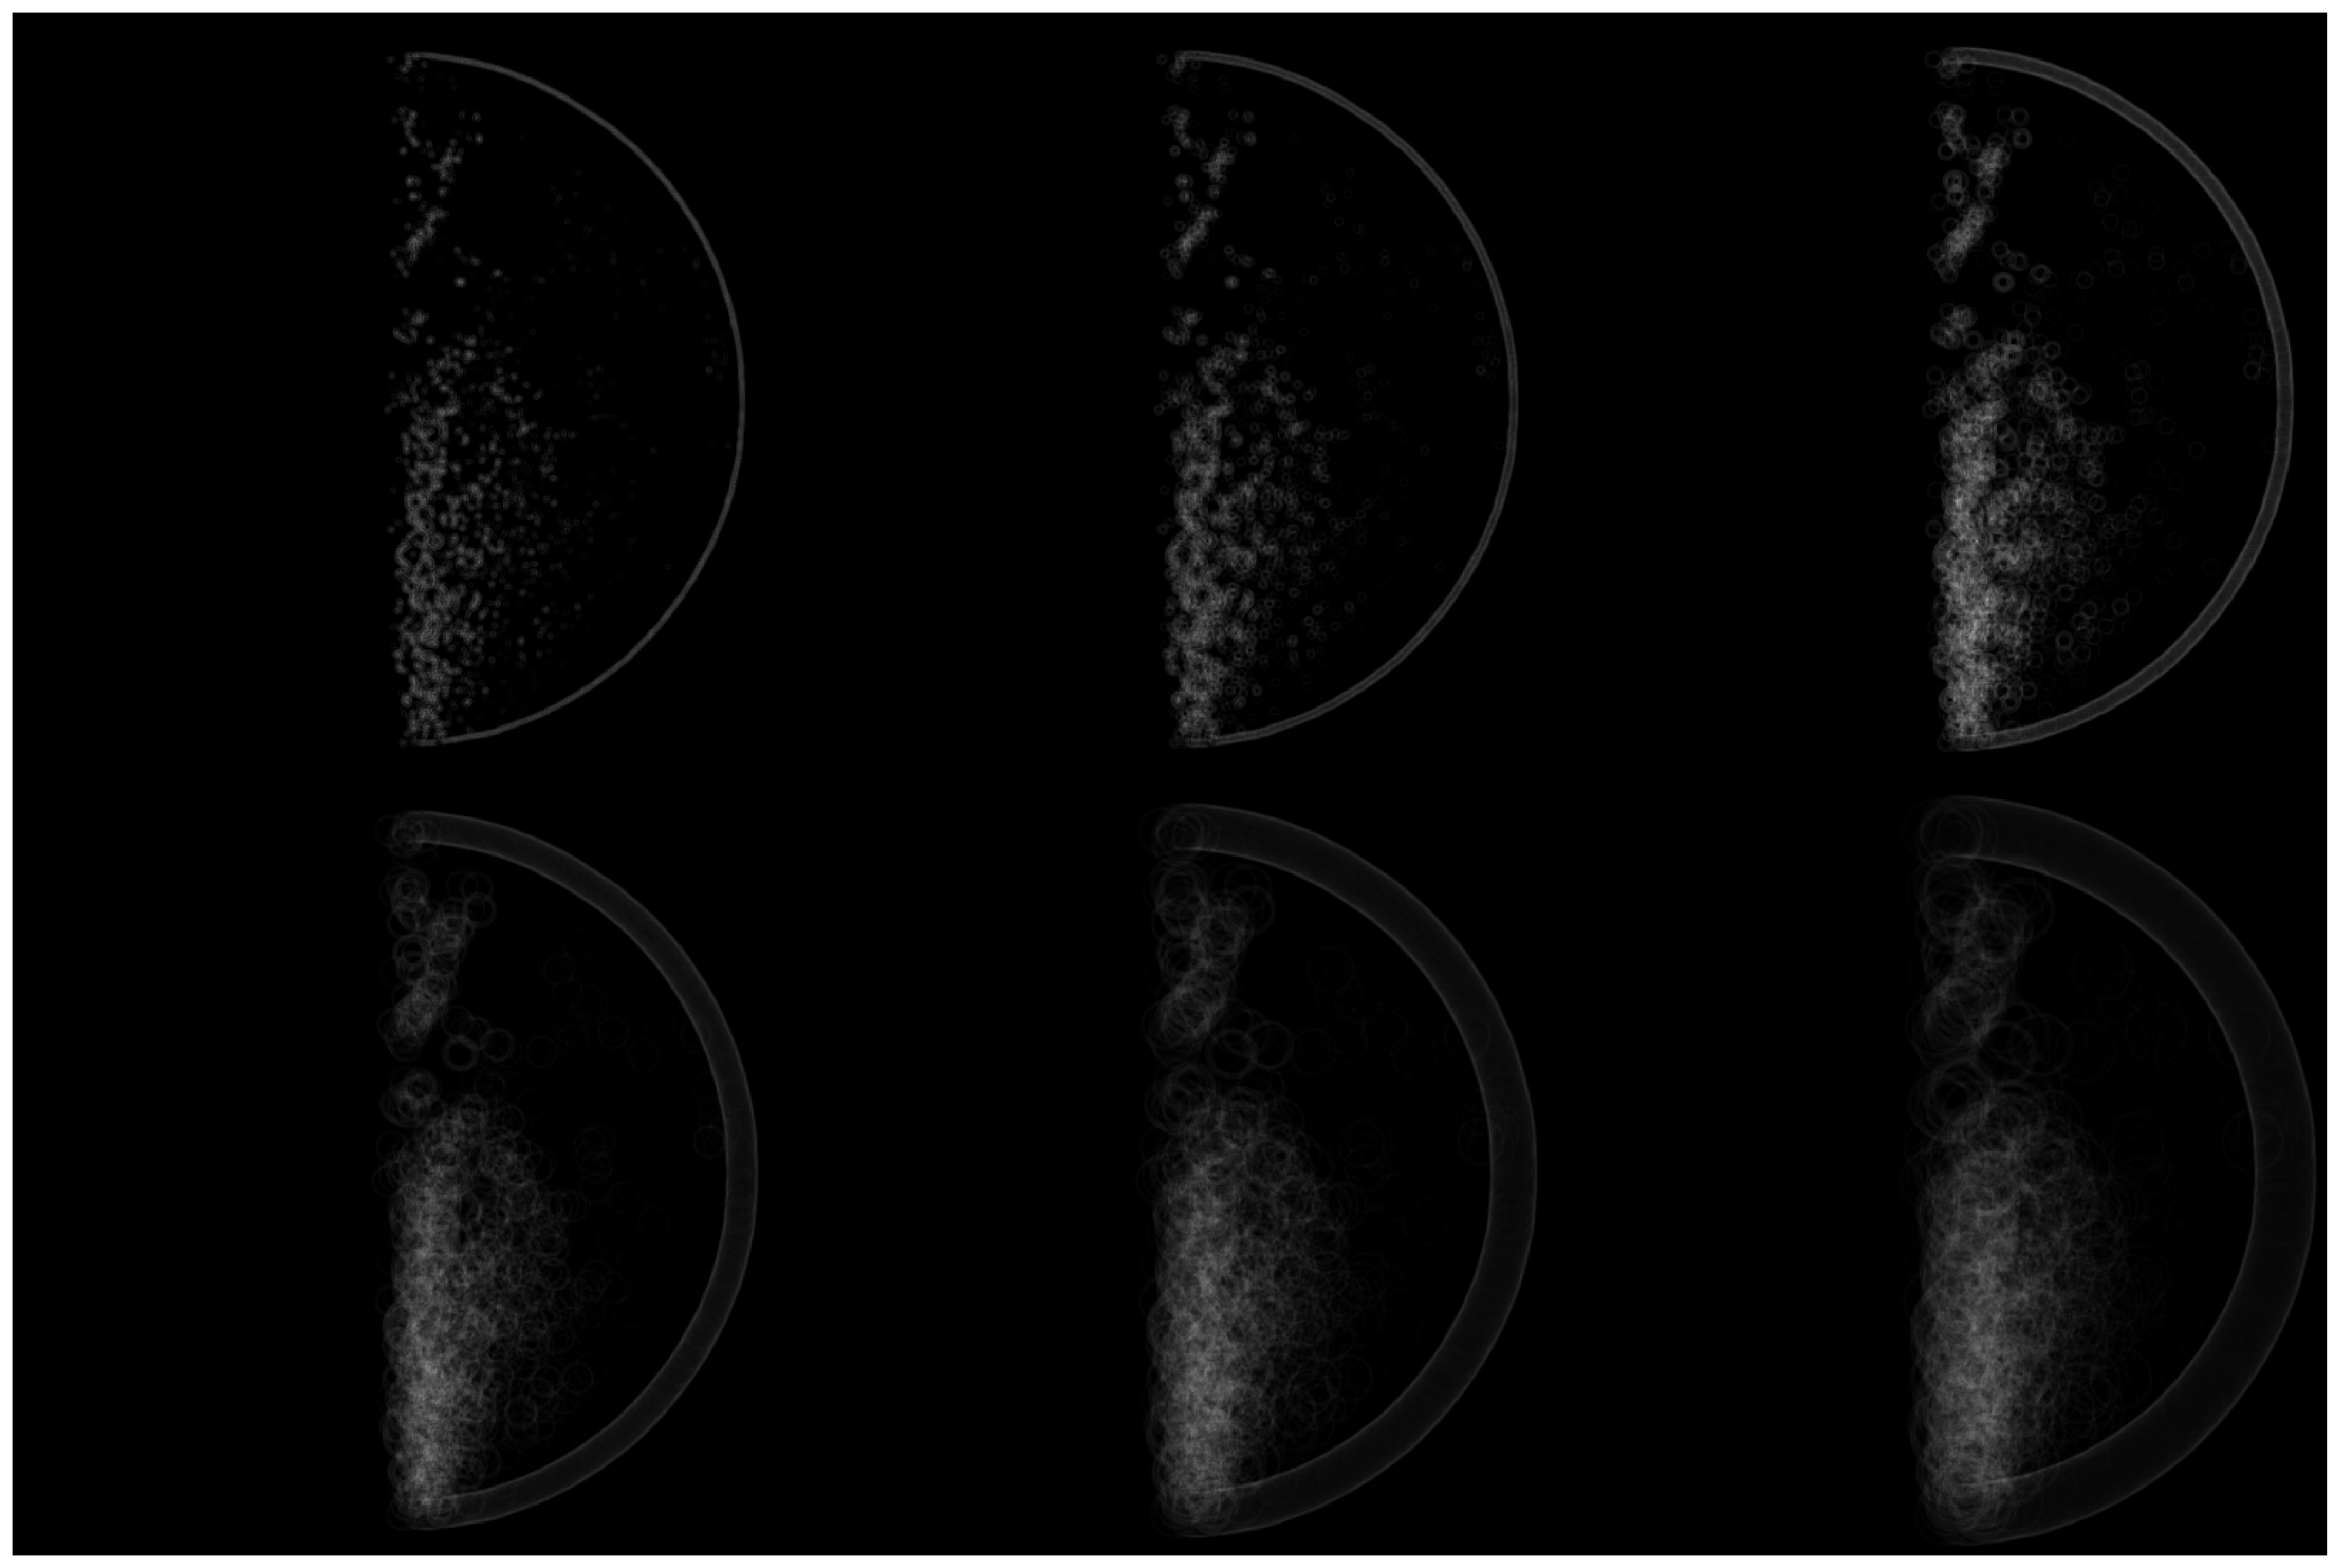
\includegraphics[width=180mm]{u10/moons.eps}
\end{center}
\label{moons}
\caption{Ergebnis ($r=3,5,10,20,30,40$)}
\end{figure}


\end{document}
